\section{Interazione con gli LLMS}
Durante lo sviluppo di questo progetto abbiamo utilizzato diversi LLMs in particolare
\textbf{ChatGpt}, \textbf{Copilot} e \textbf{Gemini}. L'utilizzo di questi strumenti è stato molto 
utile per risolvere errori, dubbi sulla progettazione e per generare il codice delle \textit{CriteriaQuery}.
Abbiamo notato che se nel prompt includiamo il contesto, dettagli, codice di riferimento ed obbiettivi precisi e specifici
si ottengono risultati migliori rispetto al caso in cui uno o più di questi elementi non vengano inclusi.
Nonostante questi accorgimenti è capitato che il LLMs in questione sbagliasse a generare la risposta alcune volte anche in modo clamoroso.
Per esempio la prima volta che abbiamo chiesto a \textbf{Copilot} di generare le classi del Domain model a partire dall'uml esso 
si è inventato un domain model tutto suo che non aveva niente in comune con il nostro.
Di seguito si riportano alcuni esempi di interazione.
\begin{figure}
    \centering
    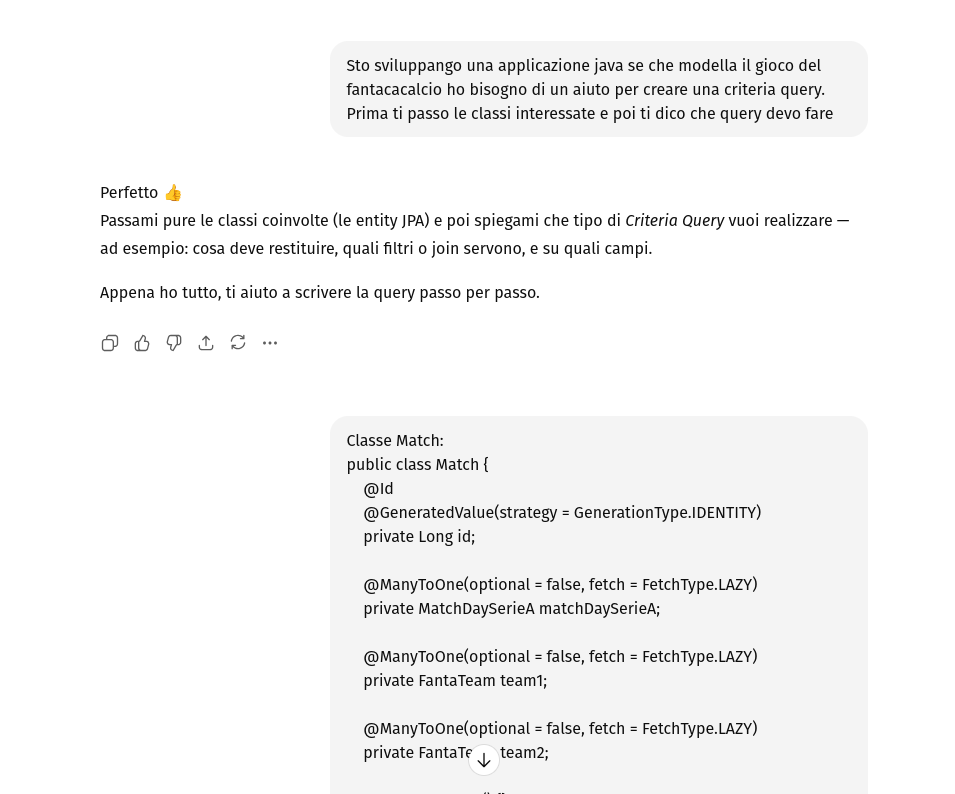
\includegraphics[width=\textwidth]{Resources/InterazioneLLMS/InterazioneParte1.png}        
    \caption{Interazione con LLMS parte 1.}
    \label{fig:interazione_con_LLMS_parte_1}
\end{figure}
\begin{figure}
    \centering
    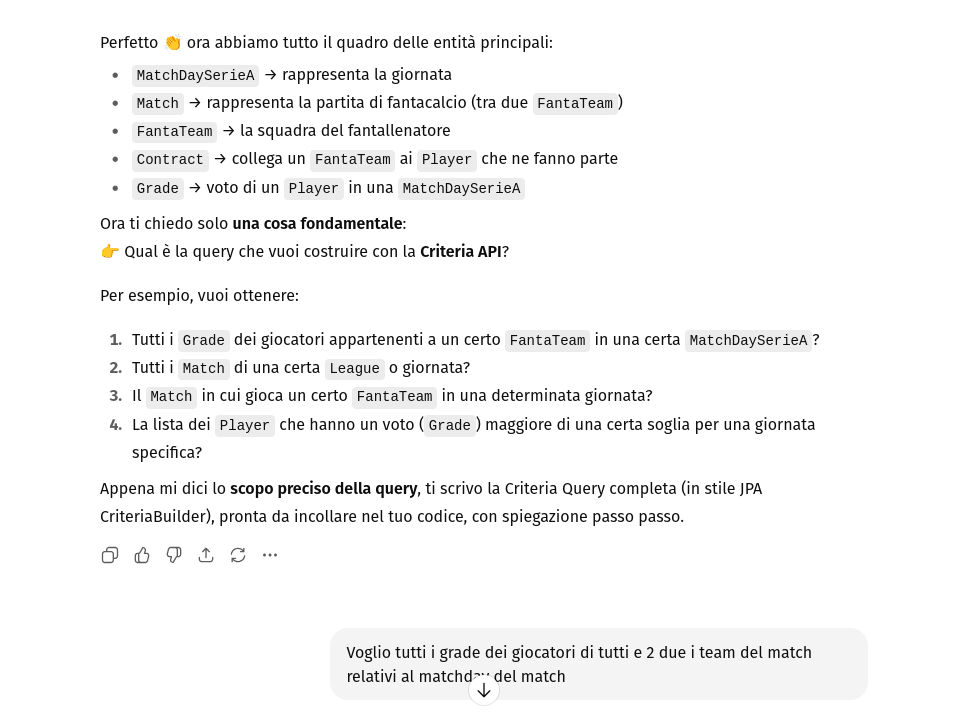
\includegraphics[width=\textwidth]{Resources/InterazioneLLMS/InterazioneParte2.png}        
    \caption{Interazione con LLMS parte 2.}
    \label{fig:interazione_con_LLMS_parte_2}
\end{figure}
\begin{figure}
    \centering
    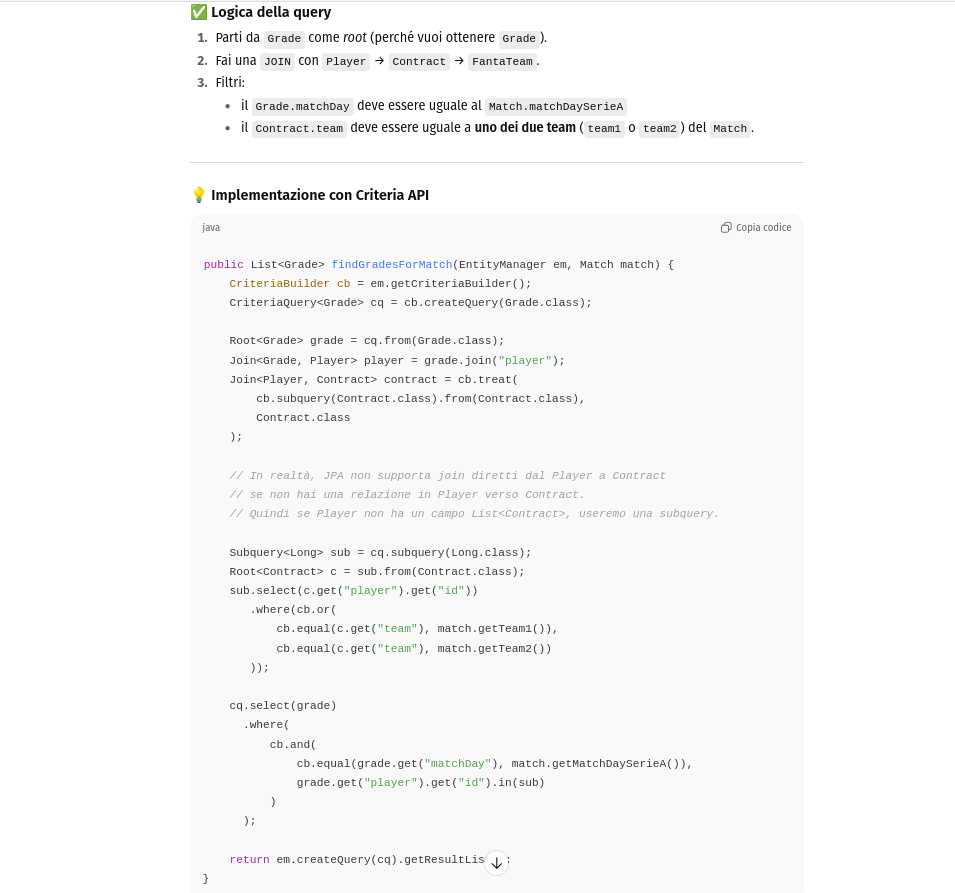
\includegraphics[width=\textwidth]{Resources/InterazioneLLMS/InterazioneParte3.png}        
    \caption{Interazione con LLMS parte 3.}
    \label{fig:interazione_con_LLMS_parte_3}
\end{figure}
\begin{figure}
    \centering
    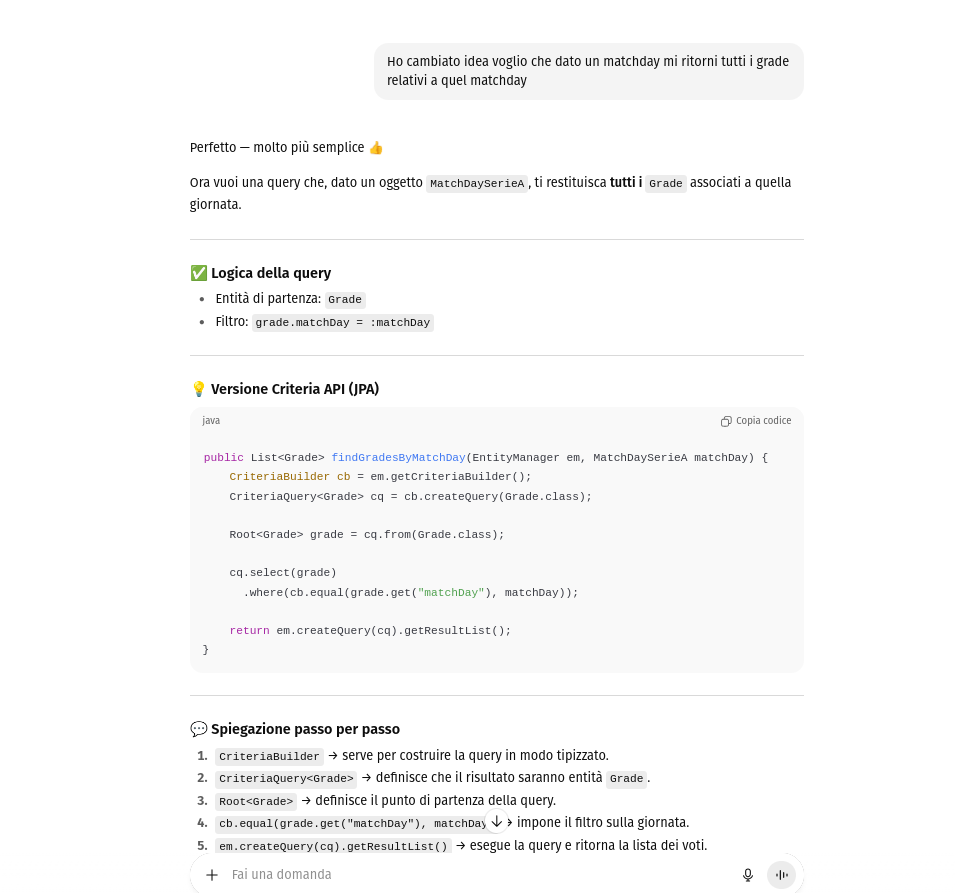
\includegraphics[width=\textwidth]{Resources/InterazioneLLMS/InterazioneParte4.png}        
    \caption{Interazione con LLMS parte 4.}
    \label{fig:interazione_con_LLMS_parte_4}
\end{figure}
